\documentclass[10pt]{beamer}
%%
\usepackage{pgfpages}
\usepackage{graphicx}
\usepackage{ulem}
\usepackage{color}
\usepackage{fancyvrb}
% get rid of junk
\usetheme{default}
\beamertemplatenavigationsymbolsempty
\hypersetup{pdfpagemode=UseNone} % don't show bookmarks on initial view
% font
\usefonttheme{professionalfonts}
\usefonttheme{serif}
% page number
\setbeamertemplate{footline}{%
    \raisebox{5pt}{\makebox[\paperwidth]{\hfill\makebox[20pt]{\color{gray}
          \scriptsize\insertframenumber}}}\hspace*{5pt}}
% add a bit of space at the top of the notes page
  \addtobeamertemplate{note page}{\setlength{\parskip}{12pt}}

\setbeamertemplate{blocks}[rounded][shadow=true]

\AtBeginSection{
\begin{frame}
\begin{center}
\structure{\Large \insertsection}
\end{center}
\end{frame}
}


\title{HGSS Workshop : Introduction to R}
\author{Jean Monlong}
\institute{Human Genetics department}
\date{Sept 23rd, 2016}

\begin{document}



%%%%%%%%%%%%%%%%%%%%
%% Title Slide
\begin{frame}
  \centering
  \titlepage
  \begin{minipage}{.3\textwidth}
    
\includegraphics[width=\linewidth]{../imgs/hgssLogo-black.png}
  \end{minipage}
  \hspace{.02\textwidth}
  \hspace{.02\textwidth}
  \begin{minipage}{.3\textwidth}
    
\includegraphics[width=\linewidth]{../imgs/McGill-Logo1.png}
  \end{minipage}

\end{frame}




%%%%
%%%%%%%%%%%%%%%%%%%%%%%
\section{Why R ?}
%%%%%%%%%%%%%%%%%%%%%%%
%%%%

\begin{frame}{Why R ?}
  \begin{block}{Simple}
    \begin{itemize}
    \item Interpretative language (no compilation needed).
    \item No manual memory management.
    \item Vectorized.
    \end{itemize}    
  \end{block}
  \begin{block}{Free}
    \begin{itemize}
    \item Widely used, vast community of R users
    \item Good life expectancy.
    \end{itemize}
  \end{block}
  \begin{block}{Flexible}
    \begin{itemize}
    \item Open-source: anyone can see/create/modify code.
    \item Multiplatform: Windows, Mac, Unix, it works everywhere.
    \end{itemize}
  \end{block}
  \begin{block}{Trendy}
    \begin{itemize}
    \item More and more packages.
    \item More and more popular among (big) data scientist.
    \end{itemize}
  \end{block}
\end{frame}

%%%%%%%

%% \begin{frame}[fragile]{R vs other languages}
%% \begin{block}{Let's create an array, shuffle it and find where is 5.}
%% \end{block}
%%   \begin{exampleblock}{In C\ldots} 
%%   {\tiny  \begin{Verbatim}
%% #include <stdlib.h>
%% #include <time.h>   
%% int main() {
%%     int size = 10;
%%     int *elements = malloc(sizeof(int)*size);
%%     int i = 0;
%%     srand(time(NULL));
%%     for (i = 0; i < size; ++i)
%%         elements[i] = i;
%%     for (i = size - 1; i > 0; --i) {
%%         int w = rand()%i;
%%         int t = elements[i];
%%         elements[i] = elements[w];
%%         elements[w] = t;
%%     }
%%     for(i = 0; i < size; ++i) {
%%         if(elements[i] == 5)
%%             printf("%d\n", i);
%%     }
%%     free(elements);
%% } 
%% 	\end{Verbatim}
%% }
%%   \end{exampleblock}
%%   \begin{exampleblock}{In R\ldots}
%%   {\tiny  \begin{Verbatim}
%%   which(sample(0:9) == 5)
%%   \end{Verbatim}
%%   }
%%   \end{exampleblock}

%% \end{frame}

%%%%%%%

\begin{frame}{R}
  \begin{block}{Easy installation}
    \begin{itemize}
    \item Install R from  \\ \url{http://cran.r-project.org/}
      \bigskip
    \item Additionally, you can get a nice interface through Rstudio Desktop from \\ \url{http://www.rstudio.com/ide/download/desktop}
    \end{itemize}
  \end{block}
  \centering
  \bigskip
  
\includegraphics[page=1,height=.3\textheight]{../imgs/Rstudio.png}

\end{frame}

%%%%%%%

\begin{frame}{Workshop setup}
  \begin{block}{Open {\sf Rstudio}}
    \begin{itemize}
    \item Click on the bottom-left corner
    \item Type {\it rstudio}, click on {\sf Rstudio} icon.
    \end{itemize}
  \end{block}
  \begin{block}{In {\sf Rstudio}}
    \begin{itemize}
    \item On the bottom-right panel, go to {\it Documents} folder.
    \item Create one for your data and scripts. E.g. {\it Rworkshop}.
    \item Set this folder as working directory ({\it More} button).
    \item Create an empty script for today's session ({\it File}, {\it New File}, {\it R Script}).
    \end{itemize}
  \end{block}
  \begin{block}{Download today's slides and data}
    \begin{enumerate}
    \item Go to \url{http://goo.gl/SYRrmy}.
    \item Download everything.
    \item Put it in your {\it Rworkshop} folder.
    \end{enumerate}
  \end{block}

\end{frame}

\begin{frame}{Console ? Script ?}
  \begin{block}{Console}
    \begin{itemize}
    \item Where R is running.
    \item You could write and run the commands directly there.
    \end{itemize}
  \end{block}
  \begin{block}{Script}
    \begin{itemize}
    \item A text file with commands. {\it Extension: .R}.
    \item To keep a trace of your analysis.
    \item Recommended.
    \item Easy to send commands from a script to the console.
    \end{itemize}
  \end{block}
\end{frame}

\begin{frame}{When you get an error}

  \begin{block}{}
    \begin{enumerate}
    \item Read the command, look for typos.
    \item Read the error message.
    \item 1. and 2. again.
    \item Raise your hand, someone will assist you.
    \end{enumerate}    
  \end{block}
  
  \begin{block}{}
    Solving errors is an important skill to learn.
  \end{block}
  
\end{frame}







%%%%
%%%%%%%%%%%%%%%%%%%%%%%
\section{Data structure}
%%%%%%%%%%%%%%%%%%%%%%%
%%%%

\begin{frame}{Data structure - Overview}
  \begin{block}{Unit type}
    \begin{description}
      \item[numeric] Numbers, e.g. $0$, $1$, $42$, $-66.6$.
      \item[character] Words, e.g. ``male'', ``ENSG0007'',``Allez les bleus''.
      \item[logical] Binary, i.e. two possible values: {\it TRUE} or {\it FALSE}.
    \end{description}
  \end{block}
  \begin{columns}
    \begin{column}{.8\textwidth}
      \begin{block}{Structure}
        \begin{description}
        \item[vector] Ordered collection of elements of the same type.
        \item[matrix] Matrix of element of the same type.
        \item[list] Flexible container, mixed type possible. Recursive.
        %%\item[data.frame] Table-like structure, same type within a column.  Recursive.
        \end{description}
      \end{block}      
    \end{column}
    \begin{column}{.2\textwidth}
      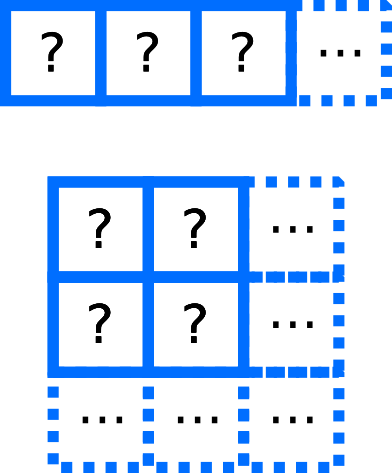
\includegraphics[width=\linewidth]{../imgs/vectorMatrixCartoon.png}
    \end{column}
  \end{columns}
\note{Other type but more complex and less useful, e.g. factors}
\end{frame}


\begin{frame}[fragile]{Assign a value to an object}
  \begin{block}{Choose an object name}
    \begin{itemize}
    \item {\bf Starts with a letter} or the dot not followed by a number.
    \item {\bf Letters}, {\bf numbers}, {\bf dot} or {\bf underline} characters.
    \item Correct: ``{\sf valid.name}'', "{\sf valid\_name}", "{\sf valid2name3}".
    \item Incorrect: "{\sf valid name}", "{\sf valid-name}", "{\sf 1valid2name3}".
    \end{itemize}
  \end{block}
  \begin{block}{Assign a value}
    The name of the object followed by the assignment symbol and the value.
    \medskip
\begin{Verbatim}[commandchars=\\\{\}]
\color{red}valid.name_123 \color{green!60!black}= \color{black}1
\color{red}valid.name_123 \color{green!60!black}<- \color{black}1

\color{red}valid.name_123
\end{Verbatim}
  \end{block}
\end{frame}

\begin{frame}[fragile]{Use a function}

  \begin{block}{}
    \begin{itemize}
    \item {\bf Parenthesis} are for {\bf functions only}.
    \item The rest will be for data manipulation.
    \item Read help manual to know more about a function ({\sf help}, {\sf ?} or {\sf F1} in Rstudio).
    \end{itemize}
  \end{block}

\bigskip

\begin{Verbatim}[commandchars=\\\{\}]
\color{red}print\color{green!60!black}(\color{black}1\color{green!60!black})
\color{red}myFunction\color{green!60!black}(\color{black}valid.name_123\color{green!60!black})

help(print)
?print
\end{Verbatim}

\end{frame}


\section{Vectors}
%%% VECTORS
%%%%%%%%%%%%%%%%%%%%
\begin{frame}[fragile]{Vectors}
  \begin{block}{{\sf vector} construction}
    \begin{description}
    \item[c] Concatenate function.
    \item[1:10] {\sf vector} with numbers from 1 to 10.
    \end{description}
  \end{block}
  \begin{exampleblock}{Example}
\begin{verbatim}
luckyNumbers = c(4,8,15,16,23,42) 
luckyNumbers
oneToTen = 1:10
tenOnes = rep(1,10)
samples = c("sampA","sampB")
samples
\end{verbatim}
  \end{exampleblock}
\note{Questions: Create your own numbers and favorite group of friends/hockey player/star/genes.\\create a vector with 10:20 and three 3\\Be creative: different names, values, sizes}

\begin{alertblock}{Extra}
  \begin{description}
  \item[seq] Create a sequence of numbers.
  \item[rep] Repeat element several times.
  \item[runif] Simulate random numbers from Uniform distribution. Same for {\sf rnorm}, {\sf rpois}, ...
  \end{description}
\end{alertblock}

\end{frame}

\begin{frame}{Exercise - Create some vectors}
  \begin{block}{Instructions}
    \begin{itemize}
    \item Create a {\sf vector} with 7 {\it numeric} values.
    \item Create a {\sf vector} with 7 {\it character} values.
    \item Be creative !
    \end{itemize}
  \end{block}
\end{frame}

%%%%%%%

\begin{frame}[fragile,shrink=5]{Vectors}
  \begin{block}{Manipulation}
    Using index/position between {\bf [ ]}.
  \end{block}
  \begin{block}{Characterization}
    \begin{description}
    \item[length] Number of element in the {\sf vector}.
    \item[names] Get or set the names of the {\sf vector}'s values.
    \end{description}
  \end{block}
  \begin{exampleblock}{Example}
\begin{verbatim}
luckyNumbers[3]
luckyNumbers[2:4]
luckyNumbers[2:4] = c(14,3,9)

length(luckyNumbers)

names(luckyNumbers)
names(luckyNumbers) = c("frank","henry","philip",
                            "steve","tom","francis") 
luckyNumbers["philip"]
\end{verbatim}
  \end{exampleblock}
  \note{Square-brackets\\Questions: \\Show me your third number\\change it\\Create a new vector with the first three numbers\\Show me the first and last values of it\\add 3 at the end of the vector\\ Name the values one two three four}
\end{frame}

%%%%%%%

\begin{frame}[fragile,shrink=5]{Vectors}
  \begin{block}{Manipulation}
    \begin{description}
    \item[sort] Sort a {\sf vector}.
    \item[sample] Shuffle a {\sf vector}.
    \end{description}
  \end{block}
  \begin{exampleblock}{Example}
\begin{verbatim}
sort(luckyNumbers)

sort(c(luckyNumbers,1:10,tenOnes))

rev(1:10)

sample(1:10)
\end{verbatim}
  \end{exampleblock}
\begin{alertblock}{Extra}
  \begin{description}
  \item[sort/sample] Explore extra parameters.
  \item[order] Get the index of the sorted elements.
  \end{description}
\end{alertblock}
\end{frame}

%%%%%%%

\begin{frame}[fragile]{Vectors}
  \begin{block}{Exploration}
    \begin{description}
    \item[head/tail] Print the first/last values.
      \medskip
    \item[{\bf\small On {\it numeric} {\sf vector}s:}]
    \item[summary] Summary statistics: minimum, mean, maximum, ...
    \item[min/max/mean/var] Minimum, maximum, average, variance.
    \item[sum] Sum of the {\sf vector}'s values.
    \end{description}
  \end{block}
  \begin{exampleblock}{Example}
\begin{verbatim}
head(samples)
summary(luckyNumbers)
mean(luckyNumbers)
min(luckyNumbers)
\end{verbatim}
  \end{exampleblock}
\begin{alertblock}{Extra}
  \begin{description}
  \item[log/log2/log10] Logarithm functions.
  \item[sqrt] Square-root function.
  \end{description}
\end{alertblock}
\note{Tips: na.rm\\Questions:\\Show me the beginning of your numbers\\average value of this beginning\\the sum of the minimum and maximum value.}
\end{frame}

%%%%%%%

\begin{frame}[fragile]{Vectors}
  \begin{block}{Arithmetic operators}
    \begin{itemize}
    \item Simple arithmetic operations over all the values of the {\sf vector}.
    \item Or values by values when using {\sf vector}s of same length.
    \item Arithmetic operation: +, -, *, /.
    \item Others exist but let's forget about them for now.
    \end{itemize}
  \end{block}
\begin{exampleblock}{Example}
\begin{verbatim}
luckyNumbers * 4
luckyNumbers - luckyNumbers
luckyNumbers / 1:length(luckyNumbers)
luckyNumbers + 2
\end{verbatim}
  \end{exampleblock}
  \note{Let's apply it to the Exercise}
\end{frame}

%%%%%%%

\begin{frame}{Exercise - Guess my favorite number}
  \begin{block}{Instructions}
    \begin{enumerate}
    \item Create a {\sf vector} with 5 {\it numeric} values
    \item Multiply it by $6$.
    \item Add $21$.
    \item Divide it by $3$ 
    \item Subtract $1$.
    \item Halve it.
    \item Subtract its original values.
    \end{enumerate}
  \end{block}
\end{frame}





%%% MATRIX
%%%%%%%%%%%%%%%%%%%%
\section{Matrix}

\begin{frame}[fragile]{Matrix}
  \begin{block}{Specific to matrices}
    \begin{description}
    \item[matrix] Create a {\sf matrix} from a {\sf vector}. \\$2^{nd}$ and $3^{rd}$ parameters define the number of rows and columns.
    \item[{mat[i,j]} ] Element at row $i$ and column $j$. If blank, the entire row/column is used.
    \end{description}    
  \end{block}
  \begin{columns}
    \begin{column}{.7\textwidth}
  \begin{exampleblock}{Example}
\begin{verbatim}
neo = matrix(1:12,3,4)
neo

neo[1,1] = 0
neo[1:2,1:3]
neo[1:2,1:3] = matrix(rep(1,6),2,3)
neo[1,]
\end{verbatim}
  \end{exampleblock}
    \end{column}
    \begin{column}{.3\textwidth}
      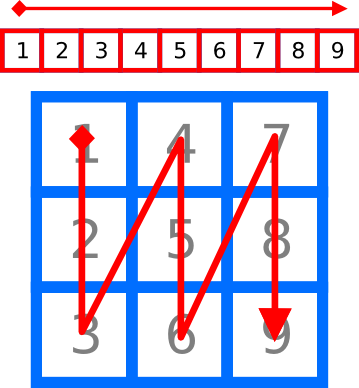
\includegraphics[width=\linewidth]{../imgs/matrixFillUpScheme.png}
    \end{column}
  \end{columns}
  \note{Questions: \\create 4x4 matrix with number from 1 to 16\\ the same but shuffled\\print the first column\\ the three first columns}
\end{frame}

\begin{frame}{Exercise}
  \begin{enumerate}
  \item Create a {\sf matrix} with 10 rows and 4 columns with numbers from 1 to 40. 
  \item Change the element in row 6 column 1 into the value 666.
  \item Fill the 3rd row with ones.
  \end{enumerate}
  \note{What if it had 100 rows...}
\end{frame}

%%%%%%%

\begin{frame}[fragile, shrink=5]{Matrix}
  \begin{block}{Specific to matrices}
    \begin{description}
    % \item[rbind/cbind] Concatenate {\sf vector}s or {\sf matrix} by row or column.
    \item[dim] Dimension of the {\sf matrix}: number of rows and columns.
    \item[rownames/colnames] Get or set the names of the rows/columns.
    \end{description}    
  \end{block}
  \begin{exampleblock}{Example}
% rbind(neo, neo)
% cbind(neo, neo)
\begin{verbatim}
dim(neo)
dim(rbind(neo,neo))

colnames(neo) = c("gene1","gene2","gene3","gene4")
rownames(neo) = c("sample1","sample2","sample3")
neo
neo["sample2","gene3"]
\end{verbatim}
  \end{exampleblock}
  \note{Questions: Add an extra line to the matrix\\Add an extra line to the matrix then the matrix\\ square matrix\\Print the new dimension}
\end{frame}

%%%%%%%

\begin{frame}[fragile]{Matrix}
  \begin{block}{Same as {\sf vector}}
    \begin{itemize}
    \item {\sf length}, {\sf head}, {\sf tail}.
    \item For {\it numeric} {\sf matrix}: {\sf min}, {\sf max}, {\sf sum}, {\sf mean}.
    \item Arithmetic operations: +, -, *, /.
    \end{itemize}
  \end{block}
  \begin{exampleblock}{Example}
\begin{verbatim}
head(mat)
mean(mat)
sum(mat) / length(mat)

mat * 2
mat + mat
\end{verbatim}
  \end{exampleblock}
\begin{alertblock}{Extra}
  \begin{description}
  \item[log/log2/log10] Logarithm functions.
  \item[sqrt] Square-root function.
  \end{description}
\end{alertblock}
  \note{Questions:\\Average of the matrix\\Average of the first two columns\\
  multiply by 2 and subtract the matrix}
\end{frame}

%%%%%%%

\begin{frame}{Exercise}
  \begin{enumerate}
  \item Create a {\sf matrix} with 100 rows and 4 columns with random numbers inside. {\scriptsize\it Tip: {\sf runif} function for random numbers.}
  \item Name the columns. E.g. {\it sampleA}, {\it sampleB}, ...
  \item Add 2 to the first column.
  \item Multiply the second column by 4.
  \item Find which column has the largest mean value.
  \item Find which column has the largest value.
  \end{enumerate}
  \note{What if it had 100 rows...}
\end{frame}

%%%%%%%

\begin{frame}[fragile]{Functions - {\sf apply}}
  \begin{block}{New best friend}
    \begin{itemize}
    \item Apply a function to each row (or column) of a {\sf matrix}.
    \item No manual iteration, the loop is implicit.
    \item Second parameter: $1$ means rows, $2$ means columns.
    \end{itemize}
  \end{block}
  \begin{exampleblock}{Example}
\begin{verbatim}
apply(mat,1,mean)
\end{verbatim}  
  \end{exampleblock}
\end{frame}

%%%%%%%

\begin{frame}{Apply - Exercise}
 
  \begin{enumerate}
  \item Create a {\sf matrix} with 100 rows and 100 columns with random numbers inside.
  \item Compute the median value of each column.
  \item What is the minimal median value ? Maximal ?
  \end{enumerate}
  
\end{frame}






%%%%
%%%%%%%%%%%%%%%%%%%%%%%
\section{Import/export data}
%%%%%%%%%%%%%%%%%%%%%%%
%%%%


\begin{frame}[fragile,shrink=10]{Import/export data - Text files}
  \begin{block}{Easy but important}
    \begin{itemize}
    \item What data structure is the more appropriate ? {\sf vector}, {\sf matrix} ?
    \item Does R read/write the file the way you want ?
    \item The extra parameters of the functions are your allies.
    \end{itemize}
  \end{block}
  \begin{block}{{\sf read.table}}
    To read a {\sf data.frame} from a multi-column file.
    \begin{description}
    \item[file=] the file name.
    \item[header=] {\it TRUE} use the first line for the column names. Default: {\it FALSE}.
    \item[as.is=] {\it TRUE} read the values as simple type, {\bf recommended}. Default: {\it FALSE}. 
    \item[sep=] the {\it character} that separate each column. Use '\t' for tabulation.
    \item[row.names=] the column number to use as row names. 
    \end{description}
  \end{block}
  \begin{exampleblock}{Example}
\begin{verbatim}
input.data = read.table("fileToRead.txt", as.is=TRUE,
                         header=TRUE, sep="\t", row.names=1)
\end{verbatim}  
  \end{exampleblock}
\end{frame}

%%%%%%%

\begin{frame}{Exercice}
  \begin{block}{Instructions}
    Read {\sf dataForBasicPlots.tsv} into an object called {\sf mat.ge}.
  \end{block}
  
  \begin{block}{{\sf dataForBasicPlots.tsv}}
    \begin{itemize}
    \item Columns separated by tabulation.
    \item First line represent the column names.
    \item First column is gene names, other columns are expression of these genes for different samples.
    \end{itemize}
  \end{block}
  
  \begin{block}{Questions}
    \begin{enumerate}
    \item How many genes are there ?
    \item How many samples ?
    \item Print the first 5 row and columns.
    \end{enumerate}
  \end{block}

\end{frame}

%%%%%%%

\begin{frame}[fragile,shrink=10]{Import/export data - Text files}
  \begin{block}{{\sf write.table}}
    To write a {\sf data.frame} in a multi-column file.
    \begin{description}
    \item[df] the {\sf matrix} or {\sf data.frame} to write.
    \item[file=] the file name.
    \item[col.names=] {\it TRUE} print the column names in the first line. Default: {\it TRUE}.
    \item[row.names=] {\it TRUE} print the rows names in the first columns. Default: {\it TRUE}.
    \item[quote=] {\it TRUE} surround {\sf character} by quotes($''$). Default: {\it TRUE} $\rightarrow$ messy. 
    \item[sep=] the {\it character} that separate each column. By default, a white-space.
    \end{description}
  \end{block}
  \begin{exampleblock}{Example}
\begin{verbatim}
write.table(resToWrite, file="fileToRead.txt", col.names=TRUE, 
                         row.names=FALSE, quote=FALSE, sep="\t")
\end{verbatim}  
  \end{exampleblock}
  \note{Questions: try to write a matrix with the different arguments\\Then re-read it.}
\end{frame}


\begin{frame}[fragile]{Import/export data}
  \begin{block}{R objects}
    \begin{description}
      \item[save] Save R objects into a file. Usual extension: {\it .RData}. {\sf file=} parameter to specify file name.
      \item[save.image] Save the entire R environment.
      \item[load] Load R objects from a ({\it .RData}) file. {\sf verbose} to print the names of the objects loaded.
    \end{description}
  \end{block}
  \begin{exampleblock}{Example}
\begin{verbatim}
save(luckyNumbers, tenOnes, mat, file="uselessData.RData")
load(file="uselessData.RData")
\end{verbatim}  
  \end{exampleblock}
  \note{Questions: load data for next exercise.\\Save your objects if you want to...}
\end{frame}

%%%%%%%








%%%%
%%%%%%%%%%%%%%%%%%%%%%%
\section{Basic plotting}
%%%%%%%%%%%%%%%%%%%%%%%
%%%%

\begin{frame}[fragile]{Basic plotting}
  \begin{block}{{\sf hist}}
    Plot the value distribution of a {\sf vector}.
    \begin{description}
    \item[x] The {\sf vector} with the values to plot.
    \end{description}
  \end{block}
  \begin{block}{{\sf plot}}
    Plot one {\sf vector} against the other.
    \begin{description}
      \item[x] The first {\sf vector} to plot. {\it x-axis}. 
      \item[y] The second {\sf vector} to plot. {\it y-axis}. 
      \item[type] How the points are plotted. ``p'' as points, ``l'' joined by lines.
    \end{description}
  \end{block}
  \begin{exampleblock}{Example}
\begin{verbatim}
hist(mat.ge[,1])
plot(mat.ge[,1],mat.ge[,2])
\end{verbatim}  
  \end{exampleblock}
\end{frame}

%%%%%%%%%

\begin{frame}[fragile]{Basic plotting}
  \begin{block}{Common parameters}
    \begin{description}
    \item[main=] A title for the plot.
    \item[xlab=/ylab=] A name for the x/y axis.
    \item[xlim=/ylim] A {\sf vector} of size two defining the desired limit on the x/y axis.
    \end{description}
  \end{block}
  \begin{exampleblock}{Example}
\begin{verbatim}
hist(mat.ge[,1],main="A basic graph",
             xlab="first column values")

plot(mat.ge[,1],mat.ge[,2],main="Another basic graph",
  xlab="first column values",ylab="second column values")
\end{verbatim}  
  \end{exampleblock}
\end{frame}

%%%%%%%%%

\begin{frame}[fragile]{Basic plotting}
  \begin{block}{Extra parameters}
    \begin{description}
      \item[col] the colour of the points/lines. 1:black, 2:red, ...
      \item[pch] Shape of the points. 1:circle, 2:triangle, ...
      \item[lty] Shape of the lines. 1:plain, 2:dotted, ...
    \end{description}
  \end{block}
  \begin{block}{Extra functions}
    \begin{description}
      \item[lines] Same as plot but super-imposed to the existent one.
      \item[abline] Draw vertical/horizontal lines.  
    \end{description}
  \end{block}
  \begin{exampleblock}{Example}
\begin{verbatim}
plot(mat.ge[,1],mat.ge[,2],main="Another basic graph",
  xlab="first column values",ylab="second column values")
lines(mat.ge[,1],mat.ge[,3],type="p",col=2,pch=2)
abline(h=0,lty=2)
\end{verbatim}  
  \end{exampleblock}
\end{frame}

%%%%%%%

%%%%%%%

%% \begin{frame}[fragile]{Basic plotting}
%%   \begin{block}{{\sf boxplot}}
%%     Plot the distribution (quantiles/median/outliers) of variables.
%%     \begin{description}
%%     \item[x] The {\sf matrix} (or {\sf list}) of distributions
%%     \end{description}
%%   \end{block}
%%   \begin{exampleblock}{Example}
%% \begin{verbatim}
%% boxplot(mat.ge)
%% \end{verbatim}  
%%   \end{exampleblock}
%% \end{frame}

%%%%%%%%%

%%%%%%%%%

\begin{frame}{Basic plotting - Exercise}
  Plot:
  \begin{enumerate}
  \item the distribution of the median gene(row) expression. Add a vertical dotted line to mark their average value.
  \item the distribution of the median sample(column) expression. If any visual outlier, remove it and check distribution again.
    {\tiny Tips: {\sf which.min} and {\sf which.max} functions give the position of the minimum/maximum values.}
  \item the expression(row) of {\it gene333} against {\it gene666}. Superimpose in red triangles the expression(row) of {\it gene333} against {\it gene667}.
  \end{enumerate}
\end{frame}









%%%%%%%
\section{Conditions}
%%%%%%%

\begin{frame}[fragile]{Logical values}
  \begin{block}{Logical type}
    TRUE / FALSE values
  \end{block}
  \begin{exampleblock}{Example}
\begin{verbatim}
hgssRules = TRUE
dwight = FALSE
male = c(TRUE, FALSE, TRUE)
\end{verbatim}  
  \end{exampleblock}
\end{frame}

%%%%%%%%%%%

\begin{frame}[fragile]{Conditions}
  \begin{block}{Logical tests}
	
    \begin{description}
    \item[{\sf ==}] both values equal ?
    \item[{\sf $>$ or $>=$}] left value greater (greater or equal)
    than right value ?
	\item[{\sf $<$ or $<=$}] left value smaller (smaller or equal) than
	left value ?
    \item[!] NOT operator : negates the value.
    \item[$|$] OR operator : returns TRUE if either are TRUE.
    \item[\&] AND operator : returns TRUE if both are TRUE.
    \end{description}
  \end{block}
  \begin{exampleblock}{Example}
\begin{verbatim}
test <- 2 + 2 == 4   ## (TRUE)
!test                ## (FALSE)
test & !test         ## (FALSE)
test | !test         ## (TRUE)
\end{verbatim}  
  \end{exampleblock}
\end{frame}

%%%%%%%%%%%

\begin{frame}[fragile]{Conditions}
  \begin{block}{Vectorized operations}
  Any logical tests can be vectorized (compare 2 {\sf vector}s).
    \begin{description}
       \item[$\mid$] Is a OR operator for vectorized application.
    \item[\&] Is an AND operator for vectorized application.
    \item[which] Returns the index of the {\sf vector}s with {\it TRUE} values.
    \end{description}
  \end{block}
  \begin{exampleblock}{Example}
\begin{verbatim}
c(TRUE, TRUE) & c(TRUE, FALSE) -> TRUE, FALSE

which(5:10 == 6)
which(luckyNumbers > 2)

luckyNumbers[which(luckyNumbers>2 & luckyNumbers<10)]
\end{verbatim}  
  \end{exampleblock}
\end{frame}
%%%%%%%%%

\begin{frame}{Conditions - Exercise}
  \begin{block}{}
    \begin{enumerate}
    \item Create a vector of random integer numbers between 0 and 10.
      {\tiny Tips:}
      \begin{itemize}
      \item {\tiny 2nd and 3rd parameters of {\sf sample} function.}
      \item {\tiny OR 2nd and 3rd parameters of {\sf runif} function and {\sf round}.}
      \end{itemize}
    \item Remove values below $3$.
    \item Change to 8 any value higher than 8.
    \end{enumerate}
  \end{block}
  \begin{block}{On {\sf mat.ge}}
    Remove all genes with median expression lower than 1.
  \end{block}
\end{frame}

%%%%%%%

\begin{frame}[fragile]{Testing conditions}
  \begin{block}{{\sf if else}}
    Test a condition, if {\it TRUE} run some instruction, if {\it FALSE} something else (or nothing).
\begin{verbatim}
if( Condition ){
...   Instructions
} 
\end{verbatim}  
  \end{block}
  \begin{exampleblock}{Example}
\begin{verbatim}
luck = "none"
if(length(luckyNumbers)>3){
  luck = "a lot"
} else if(length(luckyNumbers)==3){
  luck = "some"
} else {
  luck = "not enough"
}
\end{verbatim}  
  \end{exampleblock}
\end{frame}

\begin{frame}{Conditions - Exercise}
  \begin{block}{}
    Write a {\sf if} block that automatically classify the expression of the first gene into :
    \begin{itemize}
    \item 'high' if its maximum value is higher than 4
    \item 'low' if not.
    \end{itemize}
  \end{block}
\end{frame}

%%%%%%%







%%%%%%%
\section{Functions}
%%%%%%%


\begin{frame}[fragile]{Functions}
  \begin{block}{}
    \begin{itemize}
    \item Name of the function with parameters between parenthesis.
    \item Takes input(s) and return something. E.g. {\sf mean(luckyNumbers)}.
    \end{itemize}
  \end{block}
  \begin{block}{Do your own}
    \begin{itemize}
      \item{\bf\sf function} To define functions.
      \item All the object created within the function are temporary.
      \item{\bf\sf return} Specify what will be returned by the function. 
    \end{itemize}
  \end{block}
  \begin{block}{Structure}    
    \begin{Verbatim}[commandchars=\\\{\}]
\color{green!60!black}myFunctionName \color{blue}<- function(\color{green!60!black}input.obj1\color{blue},\color{green!60!black}second.input.obj \color{blue}) \{
\color{black}...
... Instructions on 'input.obj1' and 'second.input.obj'
...
\color{blue}return(\color{green!60!black}my.output.obj\color{blue})
\color{blue}\}
  
\color{black}myFunctionName(1,c(2,4,5))
    \end{Verbatim}
  \end{block}
\end{frame}


%%%%%%%%%
\begin{frame}[fragile]{Functions - Example}
  \begin{block}{}
    Function takes a {\sf vector} as input and :
    \begin{itemize}
    \item removes values lower than 3.
    \item changes to 8 values higher than 8.
    \end{itemize}    
  \end{block}
  
  \begin{exampleblock}{Example}
\begin{verbatim}
clean.vec.fun <- function(x){
  x = x[which(x>=3)]
  x[which(x>8)] = 8
  return(x)
}  

vec110 = 1:10
vec110.cleaned = clean.vec.fun(vec110)
\end{verbatim}
  \end{exampleblock}
  
\end{frame}

\begin{frame}{Functions - Concept}
  \centering
  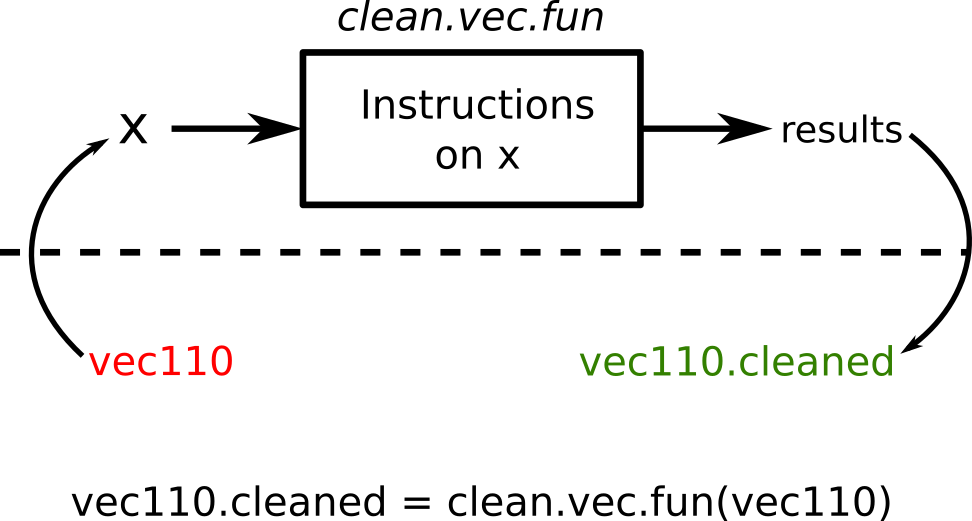
\includegraphics[width=\textwidth]{../imgs/function-cartoon.png}
\end{frame}

\begin{frame}{Functions - Exercise}
  \begin{block}{}
    Create a function that classify the average value of a {\sf vector}. It returns:
    \begin{itemize}
    \item {\it low} if the average if below $3$.
    \item {\it medium} if the average if between $3$ and $7$.
    \item {\it high} if the average if above $7$.
    \end{itemize}    
  \end{block}
  
  \begin{block}{}
    Create a function that: 
    \begin{enumerate}
    \item returns the average of the minimum and maximum value of a {\sf vector}.
    \item returns how many values are higher than 3 in a {\sf vector}.
    \end{enumerate}
  \end{block}

  \begin{block}{}
    \begin{itemize}
    \item Test your functions on {\sf vector}s with random number from 0 to 10.
    \item How would you run them on all {\sf mat.gene} genes ?
    \end{itemize}    
  \end{block}
  
\end{frame}


\begin{frame}{Final exercise}

  \begin{block}{Differential gene expression}
    \begin{enumerate}
    \item Load {\sf metadata.RData} file. It has a {\sf groups} vector with either case/control status for the {\sf mat.ge} samples.
    \item Write a function that would compute the difference between the gene expression of cases and controls.
    \item Apply this function to each gene(row) in {\sf mat.ge}.
    \item Plot the distribution of the results. 
    \end{enumerate}  
  \end{block}
  
\end{frame}


\begin{frame}[shrink=15]{Online resources}
  \begin{block}{R basics}
    \begin{itemize}
    \item \url{http://www.twotorials.com/} : small video-tutorials.
    \item \url{www.youtube.com/user/rdpeng/} : Coursera {\it Computing for Data Analysis} videos. Other interesting videos, e.g. {\it ggplot2}.
      \bigskip
    \item \url{https://www.datacamp.com/} or \url{http://tryr.codeschool.com/} : Interactive tutorial of R basics.
      \bigskip
    \item \url{http://www.r-tutor.com/} : R and statistics small web-tutorials.
    \item \url{http://www.computerworld.com/s/article/9239625/Beginner_s_guide_to_R_Introduction} : Beginner's guide with screenshots.      
    \item \url{http://cran.r-project.org/manuals.html} : R manual.
    \end{itemize}
  \end{block}
  
  \begin{block}{Bioinformatics}
    \begin{itemize}
    \item \url{http://stephenturner.us/p/edu} List of online resources for Bioinformatics.
    \item \url{http://bioinformatics.ca/workshops/2013/} : Bioinformatics workshop material.
    \item \url{http://manuals.bioinformatics.ucr.edu/home/R_BioCondManual} : Pieces of code for bioinformatics analysis, plots. Including Bioconductor.
    \item \url{http://bioconductor.org/help/course-materials/2013/} : Bioinformatics tutorials material: pdf and R scripts.
    \end{itemize}
  \end{block}


\end{frame}



%%%%%%%%%%%%%%%%%%%%%%%%%%%%%%
%%%%%%%%%%%%
%%%
\section{Extra}



\begin{frame}[fragile]{Loops}
  \begin{block}{{\sf for} loops}
    Iterate over the element of a container and run instructions.
\begin{verbatim}
for(v in vec){
...  Instruction
}
\end{verbatim}  
  \end{block}
  \begin{block}{{\sf while} loops}
    Run instructions as long as a condition is {\it TRUE}.
\begin{verbatim}
while( CONDITION ){
...  Instruction
}
\end{verbatim}  
  \end{block}
  \begin{exampleblock}{Example}
\begin{verbatim}
facto = 1
for(n in 1:10){
   facto = facto * n
}
\end{verbatim}  
  \end{exampleblock}
  \note{Apply versus loop speech then vote if they want to do the exercice?}
\end{frame}

%%%%%%%%%

\begin{frame}{Loops - Exercise}
  Write a function that computes the mean values of the columns:
  \begin{enumerate}
  \item using the {\sf apply}  function.
  \item using a {\sf for} loop.
  \item (using a {\sf while} loop.)
  \end{enumerate}
\end{frame}

\begin{frame}[fragile]{Basic plotting}
  \begin{block}{{\sf boxplot}}
    Plot the distribution (quantiles/median/outliers) of variables.
    \begin{description}
    \item[x] The {\sf matrix} (or {\sf list}) of distributions
    \end{description}
  \end{block}
  \begin{exampleblock}{Example}
\begin{verbatim}
boxplot(mat.ge)
\end{verbatim}  
  \end{exampleblock}
\end{frame}

\begin{frame}[fragile]{Save your plot into a {\it pdf/png}}
  \begin{block}{}
    Open a connection to a output file, plot as usual, close the connection.
    \begin{description}
    \item[pdf] Open the connection to a {\it pdf} output.
    \item[png] Open the connection to a {\it png} output.
    \item[dev.off()] Close the connection
    \end{description}
  \end{block}
  \begin{exampleblock}{Example}
\begin{verbatim}
pdf("myNicePlot.pdf")
plot(...)
dev.off()
\end{verbatim}  
  \end{exampleblock}
\end{frame}

%%%%%%%%%
\begin{frame}[fragile]{Type coercion.}
  \begin{block}{}
    \begin{itemize}
    \item Automatic conversion of an object to another type, e.g {\sf numeric}$\rightarrow${\sf character}, {\sf logical}$\rightarrow${\sf numeric}.
    \item Awareness for debugging.
    \item Useful sometimes.
    \end{itemize}
  \end{block}
  \begin{exampleblock}{Example}
\begin{verbatim}
is.numeric( c(1:10,"eleven") )

logical.vector = c(TRUE,TRUE,FALSE,TRUE,FALSE)
sum(logical.vector)
mean(logical.vector)
\end{verbatim}  
  \end{exampleblock}
  \note{Questions: How would you do it }
\end{frame}

%%%%%%%%%

\begin{frame}[fragile]{{\sf character} operations}
  \begin{block}{}
    \begin{description}
      \item[paste] Paste several {\it character} into one.
      \item[grep] Search a pattern in a {\sf vector} and return the index when matched.
      \item[grepl] Search a pattern in a {\sf vector} and return {\it TRUE} if found.
      \item[strsplit] Split {\it character} into several.
    \end{description}
  \end{block}
  \begin{exampleblock}{Example}
\begin{verbatim}
sample.name = "Ob5cU8eN4mE"
file.name = paste("pathToYourDirectory/greatAnalysis-",
                                sample.name,".txt",sep="")

which(sample.names=="controlA" & sample.names=="controlB")
grep("control",sample.names)
\end{verbatim}  
  \end{exampleblock}
\end{frame}

%%%%%%%%%

\begin{frame}{One-liner quiz}
  \begin{block}{Instructions}
    Write R command to address each question. Only one-line command allowed. The shorter the better.
  \end{block}
  \begin{block}{Questions}
    \begin{enumerate}
    \item From a {\sf matrix} of {\it numeric}, compute the proportion of columns with average value higher than 0.
    \item From a {\sf matrix} of {\it numeric}, print the name of the column with the highest value.
    \item From a {\sf matrix} of {\it numeric}, print the rows with only positive values.
    \end{enumerate}
  \end{block}
  \note{Find more questions.}
\end{frame}


\end{document}


%%% Local Variables:
%%% mode: latex
%%% TeX-master: t
%%% End:
